\documentclass{article}


\usepackage{arxiv}


\usepackage[utf8]{inputenc} % allow utf-8 input
\usepackage[T1]{fontenc}    % use 8-bit T1 fonts
\usepackage[hidelinks]{hyperref}       % hyperlinks
\usepackage{url}            % simple URL typesetting
\usepackage{booktabs}       % professional-quality tables
\usepackage{amsfonts}       % blackboard math symbols
\usepackage{nicefrac}       % compact symbols for 1/2, etc.
\usepackage{microtype}      % microtypography
\usepackage{authblk}
\usepackage{lipsum}
\usepackage{tikz}
\usepackage{dsfont}
\usepackage{amsmath}
\usepackage{array}
\usepackage{todonotes}
\usepackage{float}
\usepackage{rotating}
\usepackage[toc,page]{appendix} %appendix
%\usepackage[sort&compress,square,comma,authoryear]{natbib}

\usepackage{multirow, makecell}
\renewcommand{\arraystretch}{1.7}
\setlength{\tabcolsep}{12pt}

\definecolor{maroon}{RGB}{176, 48, 96}
\definecolor{orange2}{RGB}{238, 118, 0}
\newcommand{\colindic}[1]{\textcolor{maroon}{#1}}
\newcommand{\colsurvey}[1]{\textcolor{orange2}{#1}}




\title{Estimation of SARS-CoV-2 mortality during the early stages of an epidemic: a modelling study in Hubei, China and northern Italy}


\author[a]{Anthony Hauser}
\author[a]{Michel J.~Counotte}
\author[b]{Charles C.~Margossian}
\author[c]{Garyfallos Konstantinoudis}
\author[a]{Nicola Low}
\author[a]{Christian L.~Althaus}
\author[a,*]{Julien Riou}
\affil[a]{{\small Institute of Social and Preventive Medicine, University of Bern, Bern, Switzerland}}
\affil[b]{{\small Department of Statistics, Columbia University, New York, NY}}
\affil[c]{{\small MRC Centre for Environment and Health, Department of Epidemiology and Biostatistics, School of Public Health, Imperial College London, London, UK}}
\affil[*] {{\small Corresponding  author (\texttt{julien.riou@ispm.unibe.ch})}}


\begin{document}

\maketitle

\begin{abstract}
\textbf{Background.} The epidemic of severe acute respiratory syndrome coronavirus 2 (SARS-CoV-2) that originated in Wuhan, China in late 2019 is now pandemic. Reliable estimates of death from coronavirus disease 2019 (COVID-19) are essential to guide control efforts and to plan health care system requirements. The objectives of this study are to: 1) simulate the transmission dynamics of SARS-CoV-2 using publicly available surveillance data; 2) give estimates of SARS-CoV-2 mortality adjusted for bias in the two regions with the world’s highest numbers of confirmed Covid-19 deaths: Hubei province, China and northern Italy. 

\textbf{Method and Findings.} We developed an age-stratified susceptible-exposed-infected-removed (SEIR) compartmental model describing the dynamics of transmission and mortality during the SARS-CoV-2 epidemic. Our model accounts for two biases; preferential ascertainment of severe cases and delayed mortality (right-censoring). We fitted our transmission model to surveillance data from Hubei province (1 January to 11 February 2020) and northern Italy (8 February to 3 March 2020). Overall mortality among all symptomatic and asymptomatic infections was estimated to be 3.0\% (95\% credible interval: 2.6-3.4\%) in Hubei province and 3.3\% (2.0-4.7\%) in northern Italy. Mortality increased with age; we estimate that among 80+ year olds, 39.0\% (95\%CrI: 31.1-48.9\%) in Hubei province and 89.0\% (95\%CrI: 56.2-99.6\%) in northern Italy dies or will die. Limitations are that the model requires data recorded by date of onset and that sex-disaggregated mortality was not available.

\textbf{Conclusions.} We developed a mechanistic approach to correct the crude CFR for bias due to right-censoring and preferential ascertainment and provide adjusted estimates of mortality due to SARS-CoV-2 infection by age group. While specific to the situation in Hubei, China and northern Italy during these periods, these findings will help the mitigation efforts and planning of resources as other regions prepare for SARS-CoV-2 epidemics.

\end{abstract}

\section*{Introduction}

The pandemic of severe acute respiratory syndrome coronavirus 2 (SARS-CoV-2) infection has resulted in more than 260,000 confirmed cases and 11,000 deaths, as of 20th March 2020 \cite{whoreport61}. 
The infection emerged in late 2019 as a cluster of cases of pneumonia of unknown origin in Wuhan, Hubei province, China and was named coronavirus disease 2019 (Covid-19) in January 2020 \cite{wang2020novel,huang2020clinical}. 
The largest outbreak to date is still that in China, but the number of reported deaths from Covid-19 in Italy (4,032 deaths, population 60 million) has overtaken China (3,261 deaths, population 1.4 billion) \cite{whoreport61}. 
The epidemic appears to have originated from multiple zoonotic transmission events of a coronavirus, with the animal source remaining unknown \cite{jointmission}. 
The causal agent, SARS-CoV-2, was identified in January 2020 \cite{zhou2020pneumonia,gorbalenya2020severe}. 
The transmission characteristics of SARS-CoV-2 appear to be similar to those of the 1918 pandemic influenza strain \cite{riou2020pattern}, but, at this early stage, its mortality rate is still unknown. 
During the early phase of the pandemic, reliable estimates of overall mortality, i.e. the proportion of all people with SARS-CoV-2 infection who will die from the disease are needed to plan health care capacity and for epidemic forecasting. 
Clinicians need to know age- and sex-specific mortality among symptomatic patients seeking care to assess prognosis and, in severe situations, prioritize patients with the best expected outcomes. 

The crude case fatality ratio (CFR), the number of reported deaths divided by the number of reported cases at a specific time point, is not a reliable indicator of overall mortality \cite{whospeech,wang2020novel}. 
Other reported measures such as the confirmed, symptomatic or hospitalized CFR, based on different denominators, are sometimes used, adding confusion. 
The crude CFR can be misleading if used to assess the overall mortality because of two opposing biases \cite{Lipsitch2015,Battegay2020}. 
First, because of the delay of several weeks between disease onset and death, the number of confirmed and reported Covid-19 deaths at a certain time point does not consider the total number of deaths that will occur among already infected individuals (right-censoring). 
Second, surveillance-based Covid-19 case reports underestimate the total number of SARS-CoV-2-infected patients, because testing focuses on symptomatic individuals, and, among symptomatic cases, on patients with more severe manifestations (preferential ascertainment). 
It is often assumed that the crude CFR overestimates true mortality \cite{WorldHealthOrganization202046}, but it depends on the relative influence of the two opposing biases, so it could differ in different situations. 

Estimates of real time mortality will rely on surveillance data and require statistical adjustment because longitudinal studies of representative samples of individuals with SARS-CoV-2 infection will take too long. 
The objectives of this study are to: 1) simulate the dynamics of transmission and mortality of SARS-CoV-2 using publicly available surveillance data; 2) give corrected age-specific estimates of SARS-CoV-2 mortality among people with symptomatic infection and overall mortality in the two regions with the world’s highest numbers of confirmed Covid-19 deaths, the Hubei province of China and northern Italy. 


\section*{Methods}

\subsection*{Setting and data, Hubei province, China}

The first known case of Covid-19 has been traced back to December 1st, 2019 in Wuhan, the main city of the Hubei province of China \cite{huang2020clinical}.
The first death was reported on 11 January 2020.
Most early cases were linked to the Huanan Seafood Wholesale Market in Wuhan, which was closed on 1 January.
From this point, human-to-human transmission of SARS-CoV-2 occurred at a high rate in Wuhan and other areas of Hubei, leading to exponential growth of the reported incidence of Covid-19 cases (Figure \ref{fig:desc}A). 
On 20 January 2020, Chinese authorities implemented extensive control measures in Hubei: early identification and isolation of clinical cases, tracing and quarantining of contacts, temperature checks before accessing public areas, extension of the lunar new year holiday period, and extreme social distancing, including cancellation of mass gatherings  \cite{jointmission}. 
Three days later, a cordon sanitaire was imposed, with strict traffic restrictions. 
From 27 January, the daily incidence of cases, by date of disease onset, started to plateau, then decreased. 
The number of reported deaths started to increase after the increase in incidence, with a delay of a few weeks.

The Chinese Center for Disease Control and Prevention (China CDC) reported the number of Covid-19 cases by date of disease onset, and the age distribution of cases and deaths up 11 February 2020 in China (Figure \ref{fig:desc}B). 
We extracted these data, together with the age distribution of the Chinese population. 
Deaths counts were obtained from a repository aggregating data from Chinese public data sources \cite{nCov2019}.
We used data about the daily number of potentially infectious contacts by age group in Shanghai \cite{zhang2019patterns}. 
We extracted data about the age-specific prevalence of diabetes, chronic respiratory diseases, cardiovascular diseases and hypertension in China from the Institute for Health Metrics and Evaluation (IHME) website \cite{ihme}. 
We assumed that all data sources were applicable to the population of Hubei.

As of 11 February, after which information about date of disease onset was no longer available, there were 41,092 cases and 979 deaths; crude CFR 2.4\%. 


\begin{figure}[t]
	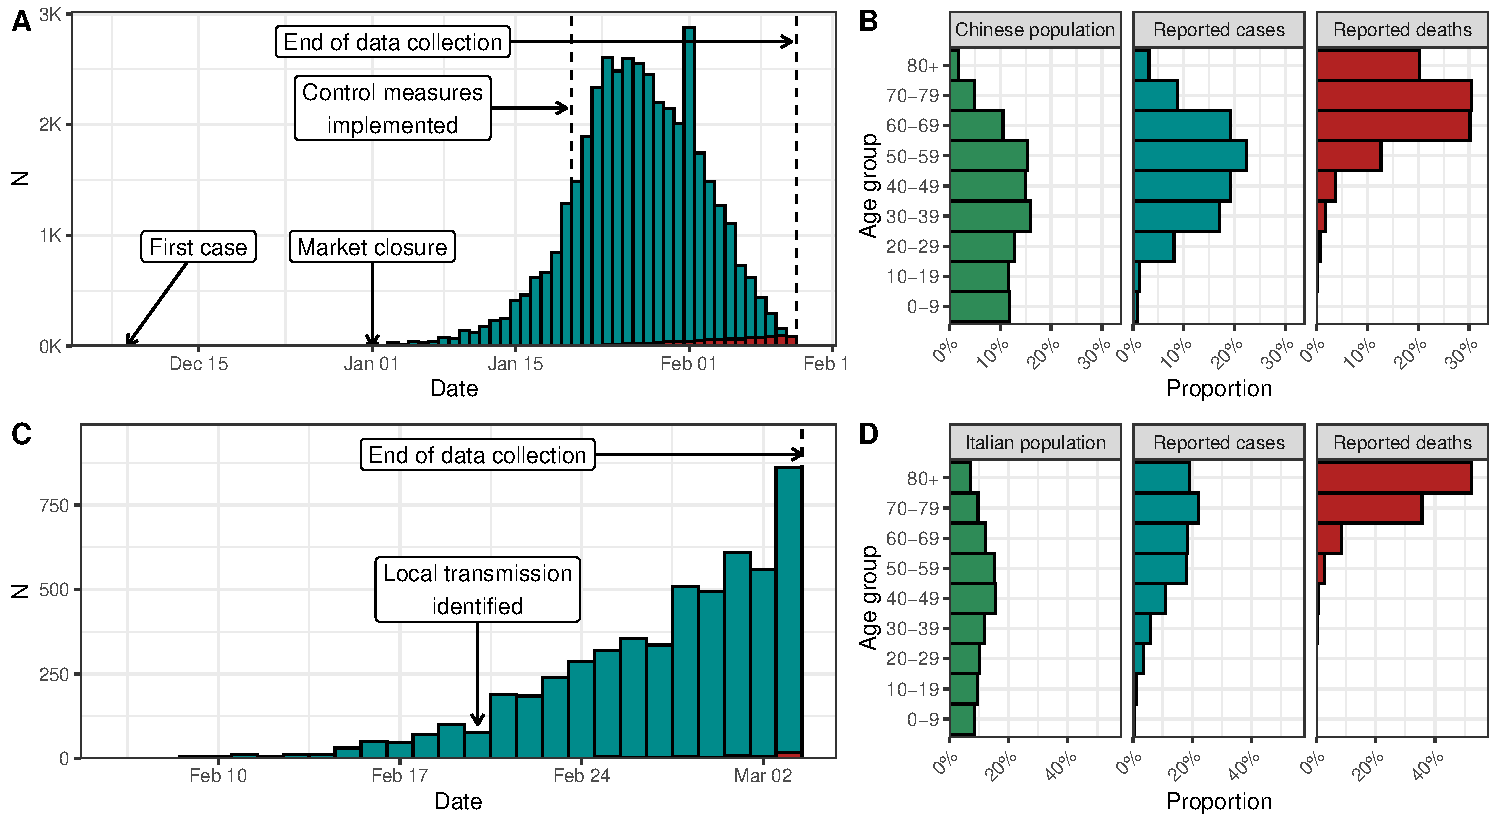
\includegraphics[width=\linewidth]{../format_output/figures/data_fig.pdf}
	\caption{(A) Reported number of Covid-19 confirmed cases by date of disease onset (blue) and of deaths (red) in Hubei, China until 11 February 2020. (B) Age distribution of the Chinese population and of the reported Covid-19 cases and deaths in Hubei, China. (C) Reported number of Covid-19 confirmed cases by date of disease onset (blue) and of deaths (red) in northern Italy until 3 March 2020. (D) Age distribution of the Italian population and of the reported Covid-19 cases and deaths in northern Italy.}
	\label{fig:desc}
\end{figure}


\subsection*{Setting and data, northern Italy}

Italy reported its first case of SARS-CoV-2 infection on 30 January 2020. 
The first reported case of local transmission was identified in 20 February in the northern region of Lombardy. 
The first death was reported on 24 February 2020.
In the following days, new cases were reported in Lombardy and the local authorities put the whole region under strict quarantine. 
Despite this, Italy faced an exponential growth of new SARS-CoV-2 infection cases (Figure \ref{fig:desc}C). 
The Italian government implemented control measures in the the whole country from 9 March, restricting movement of the population and banning public events. 

We collected data from reports from the Instituto Superiore di Sanita and the Dipartimento della Protezione Civile, which reported the number of new cases and deaths per day by date of disease onset from 8 February to 3 March, and their distribution by age group \cite{Civile,IstitutoSuperiorediSanita} (Figure \ref{fig:desc}C-D). 
We also collected data about the age distribution of the Italian population, and contact patterns, by age group, from the POLYMOD study \cite{mossong2008social}.

As of 3 March 2020, there were 6,117 cases and 79 deaths; crude CFR 1.3\%.
Further details about the data sources are available in S1 Text, section 1. 




\section*{Age-structured model of SARS-CoV-2 transmission and mortality}

We used an age-stratified susceptible-exposed-infected-removed (SEIR) compartmental model, with a distinction between incubating, asymptomatic and symptomatic infections. 
We stratified the population into nine 10-year groups (0-9 up to 80+ years). 
We assumed that susceptibility to SARS-CoV-2 and the risk of acquisition per contact is identical for each age class. 
We used age-specific contact matrices for each country to model contact patterns according to age class. 
In addition, we modelled the decrease in the transmission of SARS-CoV-2 due to the progressive implementation of control measures in Hubei from 20 January by using a logistic function for the transmission rate. 
In northern Italy we did not include the effect of control measures.

In the model, after an average incubation period of 5.9 days \cite{Bi2020}, 82.1\% (95\%CrI: 79.8-84.5) of infected people develop symptoms of any severity and become infectious, while the remainder are asymptomatic and do not transmit the infection.
The proportion of symptomatic infections is derived from data from passengers of the ``Diamond Princess'' cruise ship, implemented as a beta distribution to propagate uncertainty \cite{mizumoto2020estimating}. 
These data did not provide conclusive evidence of an age trend in the proportion of true asymptomatics, so we assumed it to be constant across age groups \cite{JapaneseNationalInstituteofInfectiousDiseases2020}.
The mean time from disease onset to isolation was fixed to 2.4 days \cite{Bi2020}.

The SEIR model was used to compute the number of symptomatic and asymptomatic SARS-CoV-2 infections by day of disease onset in each age class.
We then used an age-specific ascertainment proportion to estimate the cumulative number of symptomatic infections reported as Covid-19 cases.
To identify the parameters, we assumed that all infected patients aged 80 years and older were reported.
We assumed that mortality only occurred in symptomatic people, and that the time from disease onset to death followed a log-normal distribution with mean 20.2 days and standard deviation 11.6 \cite{linton2020incubation}.
This allowed us to account for the deaths occurring after the date of data collection (11 February for Hubei, 3 March for northern Italy). 

For Hubei and northern Italy separately, we simultaneously fitted our model to the data sets described above (Figure \ref{fig:desc}): (1) the number of confirmed cases by day of disease onset, (2) the number of deaths by day of occurrence, (3) the age distribution of all confirmed cases and (4) the age distribution of all reported deaths. 
All parameters were estimated from data except for the incubation period, the proportion of symptoms, the time from disease onset to isolation and the time from disease onset to death.
The fitted model was used to produce estimates (with uncertainty expressed as 95\% credible intervals, CrI) of the total number of symptomatic and asymptomatic infections (corrected for preferential ascertainment) and of the total number of deaths (corrected for right-censoring), which were then transformed into adjusted estimates of the mortality (per cent of all cases, with 95\% CrI).
Besides parameter values and model structure, these estimates rely on the following additional assumptions:
\begin{enumerate}
	\item The severity of symptoms differs by age group and influences the probability of reporting;
	\item All deaths due to SARS-CoV-2 infection have been identified and reported;
	\item The average standard of care is stable between the period of interest (until 11 February for Hubei, until 3 March for northern Italy) and the following period of two months during which a proportion of the infected people will eventually die;
	\item The ascertainment probability by age is constant over the periods considered.
\end{enumerate}

We implemented the model in a Bayesian framework using Stan \cite{Carpenter2017}. 
All code and data are available from \underline{\smash{\url{https://github.com/jriou/covid_adjusted_cfr}}}.
Further details about the method are available in S1 Text, section 2. 

\section*{Results}

\subsection*{Hubei province, China}

Our model accurately describes the dynamics of transmission and mortality by age group during the SARS-CoV-2 epidemic in Hubei from 1 January to 11 February 2020 (Figure \ref{fig:fit}).
The model predicts that control measures implemented from 20 January reduced SARS-CoV-2 transmissibility by 99\% (95\% credible interval [CrI]: 97-100), with a steep diminution in case incidence after six days. 
The model estimates that a total of 82,300 individuals (95\%CrI: 73,000-91,800) were infected in Hubei between 1 January and 11 February 2020.
Of these, the number of symptomatic cases is estimated at 67,500 (95\%CrI: 59,900-74,800), 1.6 times (95\%CrI: 1.5-1.8) more than the 41,092 reported cases during that period. 
The proportion of ascertained cases showed a clear age trend, from less than 10\% under 20 years old to 93\% (95\%CrI: 87-99) in the age group 70-79 (it was assumed that the ascertainment proportion was 100\% in the age group 80+, S1 Text section 4.

The model predicts a total of 2,439 deaths (95\%CrI: 2,210-2,673) among all people infected until 11 February (compared with 979 deaths at this point).
This results in an adjusted mortality of 3.0\% (95\%CrI: 2.6-3.4) among all infected individuals (Figure \ref{fig:mortality}B).
Figure \ref{fig:mortality}A shows how the adjustment for bias affects the estimated age-specific mortality. 
Compared with the crude CFR, the adjusted mortality among all individuals infected with SARS-CoV-2 is similar or lower in the younger age classes (0-49 years old) but higher in people aged 50 years and older, reaching 32.0\% (95\%CrI: 25.3-40.1) among individuals aged 80 years and older.

Among infected individuals with symptoms, which is more relevant to the clinical situation, adjusted mortality is estimated at 3.6\% (95\%CrI: 3.1-4.1). 
Under 20 years of age, mortality among symptomatics is estimated below 1 in 1,000 and rises to between 3 to 8 per 1,000 symptomatic infections for individuals aged 20 to 49 years. 
Mortality among symptomatics is estimated to 2.5\% (95\%CrI: 1.9-3.1) among individuals aged 50-59, 8.0\% (95\%CrI: 6.6-9.5) among individuals aged 60-69, 19.2\% (95\%CrI: 15.8-22.9) among individuals aged 70-79 and reaches 39.0\% (95\%CrI: 31.1-48.9) among individuals aged 80 and more. 
The estimated prevalence of the four comorbidities is shown in Figure \ref{fig:mortality}C. 
Compared with the expected prevalence given the age-distribution of deaths associated with SARS-CoV-2 infection, we observe a higher proportion of patients with diabetes and a lower proportion with chronic respiratory disease or hypertension among Covid-19 deaths in Hubei

\begin{figure}[h]
	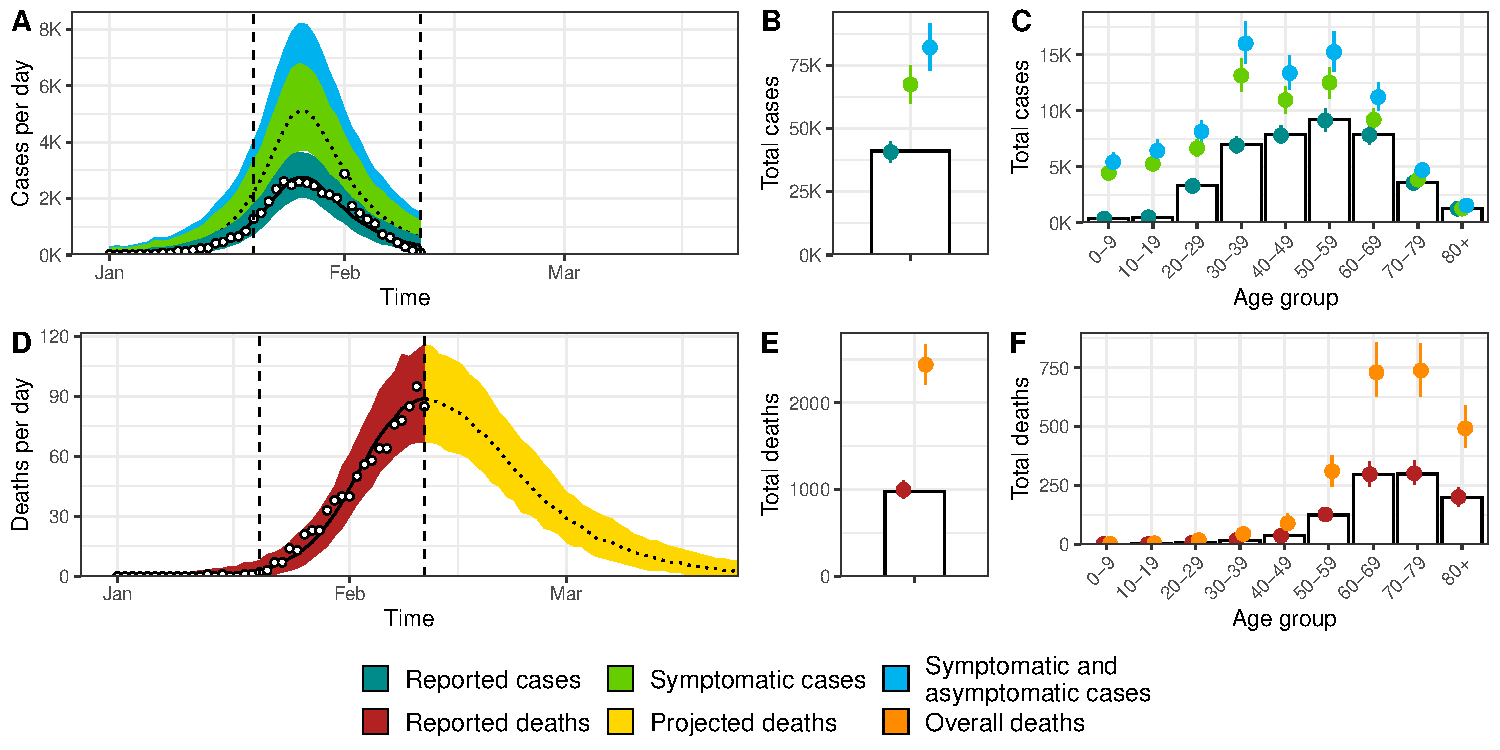
\includegraphics[width=\linewidth]{../format_output/figures/modelfit_china.pdf}
	\caption{Model fit for Hubei, China of (A) incident cases of SARS-CoV-2 infection by date of disease onset, (B) total cases, (C) age distribution of cases, (D) incidence of deaths, (E) total deaths and (F) age distribution of deaths. White circles and bars represent data. Lines and shaded areas or points and ranges show the posterior median and 95\% credible intervals for six types of model output: reported cases, symptomatic cases, overall cases (i.e. symptomatic and asymptomatic cases), reported deaths until 11 February 2020, projected deaths after 11 February 2020 and overall deaths.}
	\label{fig:fit}
\end{figure}

\begin{figure}[h]
	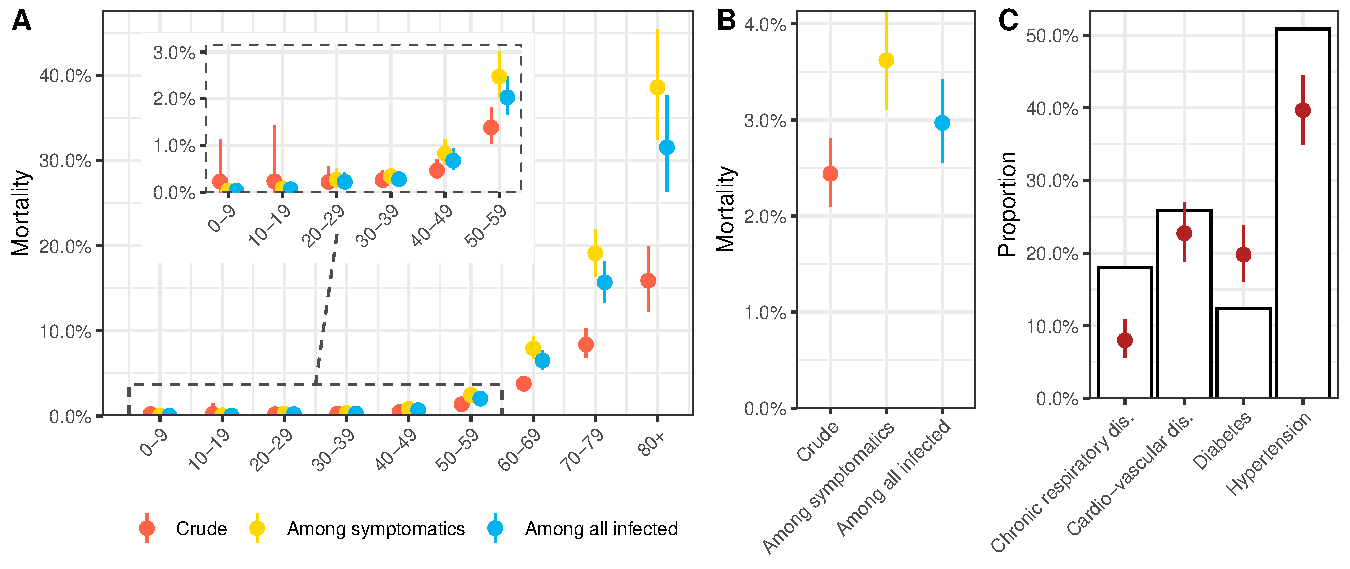
\includegraphics[width=\linewidth]{../format_output/figures/cfr_china_bis.pdf}
	\caption{(A-B) Estimates of mortality during the first wave of the SARS-CoV-2 epidemic in Hubei, China by age group and overall. (C) Observed prevalence four comorbidities among deaths associated with SARS-CoV-2 infection in Hubei (purple) compared to the expected prevalence given the age distribution of deaths and the age-specific prevalence of each comorbidity in the Chinese population (white bar). Points and ranges show the posterior median and 95\% credible intervals.}
	\label{fig:mortality}
\end{figure}



\subsection*{Northern Italy}

The model accurately describes the early dynamics of transmission and mortality by age group during the SARS-CoV-2 epidemic in northern Italy from to 2 February to 3 March 2020 (Figure \ref{fig:fitit}). 
The model predicts that a total number of 63,300 (95\%CrI: 51,000-77,200) people were infected with SARS-CoV-2 in the area until 3 March 2020.
Of these, an estimated 51,900 (95\%CrI: 41,800-63,100) were symptomatic, 8.5 (95\%CrI: 6.8-10.3) times more than the 6,117 reported cases during that period.
The proportion of ascertained cases was estimated to be 1\% in under 20 years old, rising to 62\% (95\%CrI: 58-67) in the 70-79 age group (it was assumed that ascertainment was 100\% in the 80+ age group, S1 Text section 4).

Among people infected with SARS-CoV-2 in northern Italy until 3 March, we estimate that 2,053 (95\%CrI: 1,238-2,910) will die, of which only 79 had been reported at this date.
This translates into an adjusted mortality of 4.0\% (95\%CrI: 2.4-5.7) among infected individuals with symptoms and of 3.3\% (95\%CrI: 2.0-4.7) among all people infected with SARS-CoV-2 (Figure \ref{fig:mortalityit}B).
We observe an even sharper age trend in mortality in northern Italy compared with Hubei, China, with an estimated mortality of 1.0\% (95\%CrI: 0.6-1.4) in symptomatic individuals aged 50-59, 5.4\% (95\%CrI: 3.4-6.9) in symptomatic individuals aged 60-69, 35.7\% (95\%CrI: 22.4-42.7) in symptomatic individuals aged 70-79 and 89.0\% (95\%CrI: 56.2-99.6) in symptomatic individuals aged 80 and older. 

\begin{figure}[h]
	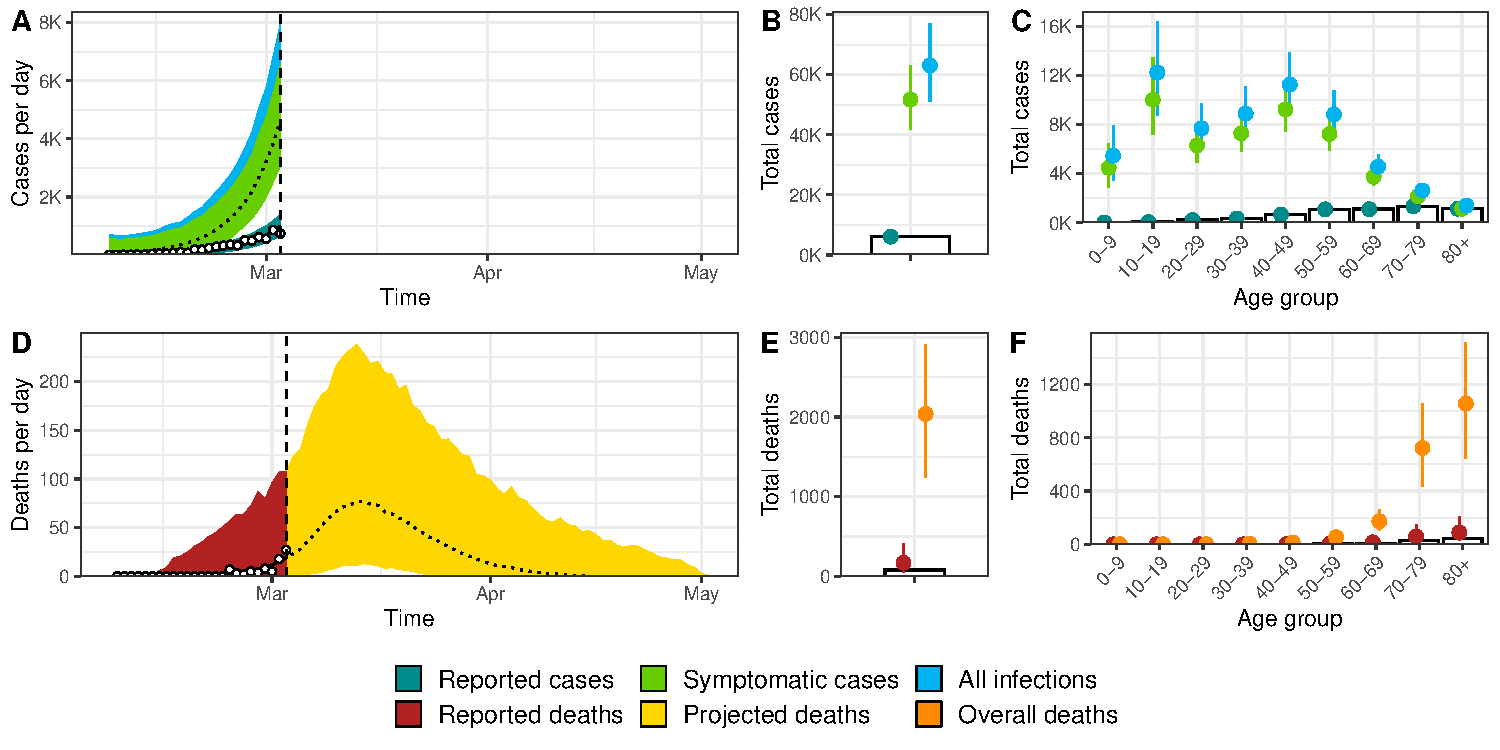
\includegraphics[width=\linewidth]{../format_output/figures/modelfit_italy.pdf}
	\caption{Model fit for northern Italy of (A) incident cases of SARS-CoV-2 infection by date of disease onset, (B) total cases, (C) age distribution of cases, (D) incidence of deaths, (E) total deaths and (F) age distribution of deaths. Coloured dots and white bars represent data. Lines and shaded areas or points and ranges show the posterior median and 95\% credible intervals for five types of model output: reported cases, symptomatic cases, overall cases (i.e. symptomatic and asymptomatic cases), reported deaths until 3 March 2020, and overall deaths including these that will occur after this date.}
	\label{fig:fitit}
\end{figure}

\begin{figure}[h]
	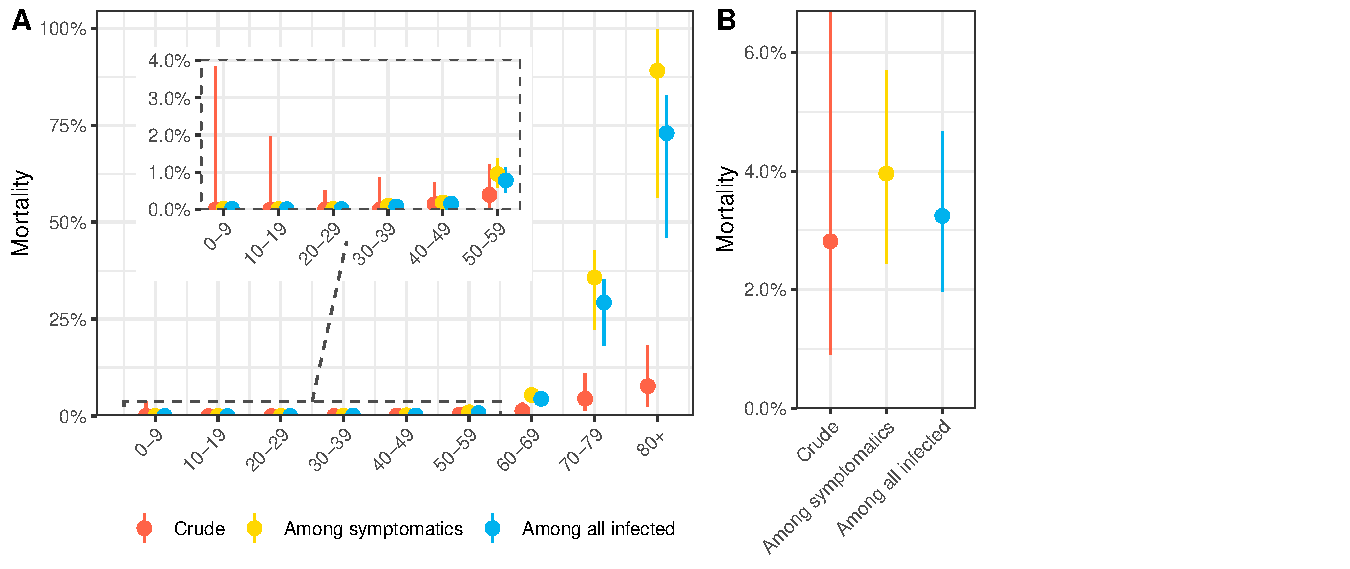
\includegraphics[width=\linewidth]{../format_output/figures/cfr_italy.pdf}
	\caption{(A-B) Estimates of mortality during the first wave of the SARS-CoV-2 epidemic in northern Italy by age group and overall. Points and ranges show the posterior median and 95\% credible intervals.}
	\label{fig:mortalityit}
\end{figure}



\section*{Discussion}


In this modelling study, we estimate mortality from SARS-CoV-2 infection and apply it to data from the SARS-CoV-2 epidemics in Hubei province, China until 11 February 2020 and in northern Italy until 3 March 2020.
After correcting for right-censoring and preferential ascertainment, we estimate mortality in the Hubei province at 3.0\% (2.6-3.4) of all individuals infected during that period, compared with a crude CFR of 2.4\%.
In northern Italy, we estimate overall mortality at 3.3\% (95\%CrI: 2.0-4.7), compared with a crude CFR of 1.3\%.
The model estimates show a strong age trend in mortality, with a sharp increase in mortality from 50 years old, reaching very high values in people aged 80 and older: 39.0\% (95\%CrI: 31.1-48.9) in Hubei province and 89.5\% (95\%CrI: 62.0-99.6) in northern Italy.
This illustrates that crude CFR values are not necessarily overestimates of true mortality, as the effect of right-censoring can be massive, especially at early stages of an epidemic.

\subsection*{Strengths and limitations}


Our work has three important strengths. 
First, we use a mechanistic model for the transmission of, and mortality associated with SARS-CoV-2 infection which directly translates the  data-generating mechanisms leading to biased observations of the number of deaths (because of right-censoring) and of cases (because of preferential ascertainment). 
Our model also accounts for the effect of control measures on disease transmission. 
We implemented the model in a Bayesian framework in order to propagate most sources of uncertainty from data and parameter values into the estimates.
In Hubei province, as the model captured most of the epidemic wave, the predicted number and timing of deaths could be compared with later reports of Covid-19 deaths, providing some degree of external validation (S1 Text, section 3).
Second, our model is stratified by age group, which has been shown as a crucial feature for modelling emerging respiratory infections \cite{pellis2020systematic}. 
Third, the model relies on routinely collected surveillance data, and does not require individual-level data or studies in the general population. 

Our results also come with several limitations. 
First, we assume that the deficit of reported cases among younger age groups is a result of preferential ascertainment, whereby younger individuals have milder symptoms and are less likely to seek care, and does not reflect a lower risk of infection in younger individuals. 
The reason for the shifted age distribution of reported cases is unclear. 
During the pandemic of H1N1 influenza, lower circulation in older individuals was attributed to residual immunity \cite{perez2009residual}. 
Lower susceptibility of younger individuals for immunological reasons seems unlikely. 
There is no indication of pre-existing immunity to SARS-CoV-2 in humans \cite{jointmission}. 
Different contact patterns could contribute to different attack rates by age group, but we include age-specific contact patterns in the model. 

Second, we assume that, as a result of more severe symptoms at older ages, all cases in symptomatic individuals aged 80 years were reported. We cannot confirm this, but the high risk of death from Covid-19 amongst the elderly was reported very early on \cite{huang2020clinical}, so we believe that most old people with symptoms sought care. If this assumption is wrong, mortality in our study would be overestimated. Sensitivity analyses show a linear relation between the ascertainment proportion for the people aged 80 years and older and mortality (S1 Text, section 5).

Third, the proportion of asymptomatic infections is uncertain. Detection of asymptomatic SARS-CoV-2 infection is limited by the focus of testing on symptomatic patients seeking care. Two independent studies have obtained similar estimates using different data sources. During the outbreak on the cruise ship “Diamond Princess”, nearly all individuals were tested regardless of symptoms, leading to an average proportion of symptomatic infections of 82.1\% (95\%CrI: 79.8-84.5) of infected people develop symptoms and become infectious \cite{mizumoto2020estimating}. Another study of 87 contacts of infected cases in Shenzhen, China, estimated that 80.4\% (95\%CrI: 70.9-87.4) were symptomatic \cite{Bi2020}. Additionally, dichotomization into asymptomatic and symptomatic is a simplification; SARS-CoV-2 causes a spectrum of symptoms, likely depending on age, sex and comorbidities. Serological surveys will be needed to better characterize asymptomatic infections \cite{carrat2008time}.

\subsection*{Comparison with other studies}

Estimates of mortality from SARS-CoV-2 in China adjusting for bias vary. 
Our estimate for Hubei province is higher than the 1.38\% estimated for mainland China \cite{Verity2020}. 
Verity et al. used a similar approach to ours, but there are differences between the models. 
They considered all mainland China, where mortality appears to be lower than in Hubei province \cite{Team2020}. 
They assumed a homogeneous attack rate across age groups rather than simulating epidemics using an age-specific contact matrix, and assumed a reporting rate of only 70\% for the elderly. 
Other studies that attempt to correct for right-censoring of deaths give higher estimates of mortality than in our study. 
A study using a competing risk model estimated mortality at 7.2\% (95\% confidence interval: 6.6\%-8.0\%) for Hubei province \cite{wang2020estimating}. Using data on exported cases, another team estimated mortality of 5.3\% (95\% confidence interval: 3.5\%, 7.5\%) among confirmed cases in China \cite{jung2020real}. 
Another team reported a CFR of 18\% (95\% credible interval: 11-81\%) among cases detected in Hubei, accounting for the delay in mortality and estimated the overall CFR at 1\% (95\% CI: 0.5\%-4\%), based on data from the early epidemic in Hubei and from cases reported outside China \cite{Dorigatti}. 
Our estimate of mortality among all infected cases in Hubei is also higher than in an earlier version of this work (3.0\% against 1.6\%) \cite{riou2020adjusted}. We believe the newer estimate to be more reliable for two reasons. First, we implemented age-specific risks of transmission through a contact matrix, which partially explains the age patterns in reported Covid-19 cases and leads to lower estimates of the total number of infections, thus increasing mortality. Second, a higher estimated proportion of symptomatic people, based on new studies \cite{mizumoto2020estimating,Bi2020}, also led to higher estimates of mortality among all infected.

\subsection*{Interpretation and implications} 

In this study, we propose a comprehensive solution to the estimation of mortality from surveillance data during outbreaks \cite{Lipsitch2015}. Our findings show that the crude CFR does not necessarily overestimate true mortality. 
In both settings that we studied, the crude CFR was lower than the model-estimated mortality, showing the importance of bias due to right-censoring at early stages of the epidemic. 
The study shows the value of collecting case data according to date of disease onset.

These estimates of overall mortality among all SARS-CoV-2 infections are of interest for assessment of the potential consequences of the pandemic, e.g. using theoretical estimates of final epidemic size \cite{hethcote2000mathematics}. 
At the early stage of the epidemic, our estimates from the very different settings of Hubei province and northern Italy are very similar. 
The findings describe the situation in Hubei before 11 February and in northern Italy before 3 March 2020. 
It was demonstrated in Hubei province, that mortality rates have changed over time as a result of an improvement of the standard of care \cite{jointmission}. 
Our estimates here correspond to an average value over the considered period, and correspond well to subsequent reports (S1 Text, section 3).
In northern Italy, our model estimate of 2,053 (95\%CrI: 1,238-2,910) deaths resulting from SARS-CoV-2 cases infected up to 3 March is nearly  25 times higher than reported deaths at this point. 
The rapid increase in reported deaths from Italy after 3 March lends weight to our estimates, but indicates that the number of deaths will continue to increase for some weeks, despite strict social distancing measures.

Observing such similar estimates in very different settings may be an indication of some degree of generalizability. 
However, direct extrapolation of these estimates to other countries must be done with caution, as the pattern of an epidemic, the standard of care and, as a result, mortality are time- and setting-dependent. 
For instance, very few deaths have been reported so far in South Korea \cite{KCDC}. 
In this country, there is a large excess of young women in a cluster of SARS-CoV-2 infections associated with the Shincheonji Church of Jesus \cite{shim2020transmission}. 
The higher number of young people among cases, widespread testing and better management of the epidemic might explain the fewer numbers of reported fatalities. 
The disproportionate influence of this cluster on the age-specific distribution of cases prevented us from applying the same model based on the age distributions in the general population. 
Data from other countries, in particular the number of cases by date of disease onset and the age and gender distribution of cases and deaths, are necessary to better understand the variability in mortality across settings. 

Estimates of age-specific SARS-CoV-2-associated mortality in symptomatic patients are particularly important for clinicians, who need to assess prognosis and prioritize care when healthcare systems are overwhelmed as the case now appears in northern Italy. 
The age-specific differences in mortality can be intuitively understood by comparing the age distributions of cases and deaths in both settings (Figure \ref{fig:desc}B and D), with an even more marked age shift in Italy resulting in higher mortality estimates in that group (Figure \ref{fig:mortality}A and \ref{fig:mortalityit}A). The specific causes of this age trend are unknown, but early discussions have focused on the associations between SARS-CoV-2 and comorbidities such as diabetes and hypertension and the role of ACE inhibitors \cite{fang2020patients}. Here, we simply compared the prevalence of four comorbidities (diabetes, chronic respiratory disease, cardio-vascular disease and hypertension) among deaths associated with SARS-CoV-2 infection in China with the expected prevalence according to the age distribution of deaths. Only for diabetes was there an excess among SARS-CoV-2-associated deaths. The prevalence of the other comorbidities was similar or lower than expected in a Chinese population with that age distribution. The reliance on data that are not gender-disaggregated means that hypotheses about the potential influence of gender-related differences like smoking patterns could not be explored. This ecological observation does not refute any causality between these comorbidities and SARS-CoV-2-related mortality, as the age trend itself may be related to a higher prevalence of ageing-associated diseases, but highlights that the very specific age pattern of mortality associated with SARS-CoV-2 infection must be accounted for when discussing association with comorbidities.

\section*{Conclusions}

We developed a mechanistic approach to correct the crude CFR for bias due to right-censoring and preferential ascertainment and provide adjusted estimates of mortality due to SARS-CoV-2 infection by age group and according to symptom status. The adjusted estimates of mortality in Hubei province, China and northern Italy were similar, and higher than the crude CFR, suggesting that, in these settings at these times, right-censoring is a more important source of bias than preferential ascertainment. The steep increase in mortality among people aged 60 years and older, reaching extremely high values in people aged 80 years and older is of concern. 
While specific to the situation in Hubei, China and northern Italy during these periods, these findings will help the mitigation efforts and planning of resources as other regions prepare for SARS-CoV-2 epidemics.


\bibliography{sup_bib}
\bibliographystyle{unsrt}  


\section*{Acknowledgements}

We warmly thank Ben Bales for his help with the implementation of the model. We also thank all the people that collected this data and made it public.

\section*{Funding}

JR is funded by the Swiss National Science Foundation (grant 174281). MC is funded by the Swiss National Science Foundation (grant 176233).

\section*{Conflict of interest}

None.

\section*{Authors' contributions}

AH and JR designed the study. 
AH, MC, CM and JR implemented the model and performed the statistical analyses. 
AH, MC, CM, GK, NL, CA and JR interpreted the results and wrote the manuscript.

\end{document}
